\chapter[TKM: a temporal knowledge model]{A temporal knowledge meta-model to represent, reason and diagnose decisions, their circumstances and their impacts}
\chapterPage{
Adaptation processes are executed with a high frequency to react to any incident whereas the delay for decision applications are constrained by the time to execute the delayed actions.
We identified two problems that result from these different paces.
First, not considered unfinished actions, together with their expected effects, over time lead upcoming analysis phases potentially make suboptimal decisions.
Second, explanations of adaptation processes remain challenging due to the lack of tracing ability of current approaches.
To tackle this problem, we first propose a knowledge formalism to define the concept of a decision. 
Second, we describe a novel temporal knowledge model to represent, store and query decisions as well as their relationship with the knowledge (context, requirements, and actions).
We validate our approach through a use case based on the smart grid at Luxembourg.
We also demonstrate its scalability both in terms of execution time and consumed memory.
 }
 
 \section{Introduction}

%% Research questions
\paragraph{Delayed actions}
General research question:
\begin{center}
	\textbf{RQ1}: Do current state of the art solutions allow modeling and reasoning over delayed actions?  
\end{center}

Sub research questions:
\begin{itemize}
	\item \textbf{RQ1.1}: How current approaches model the evolution of the context and/or the evolution of the behavior of systems over time?
	\item \textbf{RQ1.2}: Do these solutions model actions, their circumstances and their effects?
	\item \textbf{RQ1.3}: What are the solutions that enable the reasoning over the evolving context and/or behavior of systems?
\end{itemize}


\paragraph{Uncertainty}

%% Methodology
Snowballing approach~\cite{DBLP:conf/ease/Wohlin14}

\paragraph{Inclusion criteria}
\begin{itemize}
	\item \textbf{IC1}: The paper has been published before the May 31 2019
	\item \textbf{IC2}: The paper is available online and written in English
	\item \textbf{IC3}: The paper describes a modeling approach that abstract the context or behavior of a system.
	\item \textbf{IC4}: The paper describes an approach that enables to reason or navigate through a temporal model.
\end{itemize}

\paragraph{Exclusion criteria}
\begin{itemize}
	\item \textbf{EC1}: The paper has less than 4 pages (short paper).
	\item \textbf{EC2}: The paper presents a work in progress (workshop papers), a poster, vision or doctoral studies.
	\item \textbf{EC3}: The paper describes a secondary study (\eg literature reviews, lessons learned).
	\item \textbf{EC4}: The document has not been published in a venue with a peer-review process. For example, technical and research report or white papers.
	\item \textbf{EC5}: The document is an introduction to the proceedings of a venue or a special issue.
\end{itemize}

However, the references of papers rejected are considered for the snowballing iteration.
 \section{Knowledge formalization}
\label{sec:tkm:k-formalism}
 
As discussed previously, we consider \gls{knowledge} to be the association of \gls{context} information, \glspl{requirement}, and \gls{action} information, all in one global and unified model.
 While \gls{context} information captures the state of the system environment and its surroundings, the system \glspl{requirement} define the constraints that the system should satisfy along the way. 
 \Glspl{action}, on the other hand, are meant to reach the goals of the system.
  
 In this section, we provide a formalization of the \gls{knowledge} used by adaptation processes based on a temporal graph. 
Indeed, due to the complexity and interconnectivity of system entities, graph data representation is an appropriate way to represent the \gls{knowledge}. 
Augmented with a temporal dimension, temporal graphs are then able to symbolize the evolution of system entities and states over time. 
We benefit from the well-defined graph manipulation operations, namely temporal graph pattern matching and temporal graph relations to represent the traceability links between the \glspl{decision} made and their \glspl{circumstance}.

Before describing this formalism, we describe the semantics used for the temporal axis.
Then, we exemplify the knowledge formalism using the Luxembourg smart grid use case, detailed in Section~\ref{sec:tkm:intro:uc}.

\subsection{Formalization of the temporal axis}
\label{sec:tkm:k-formalism:timeAxis}

\begin{figure}
   \centering
	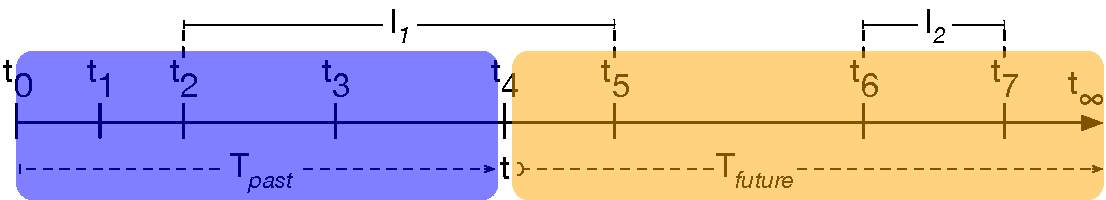
\includegraphics[width=\textwidth]{img/chapt-tkm/formalism/formalismeTime}
	\caption{Time definition used for the knowledge formalism}
	\label{fig:tkm:formalismeTime}
\end{figure}

The formalism described below has been made with two goals in mind.
First, the definition of the time space should allow the distinction between past and future. 
Doing this distinction enable the differentiation between measured data and predicted (or planned data).
Second, it should permit the definition of the life cycle of an element of the \gls{knowledge}, which can be seen as a succession of states with a validity period that should not overlap each other.

Time space $T$ is considered as an ordered discrete set of time points non-uniformly distributed. 
As depicted in Figure~\ref{fig:tkm:formalismeTime}, this set can be divided into 3 different subsets $T = T_{past} \cup \{t\} \cup T_{future}$, where:   \begin{itemize}  \item $T_{past}$ is the subdomain \{$t_{0}$;$t_{1}$;\ldots;$t_{current-1}$\}  representing graph data history starting from $t_0$, the oldest point, until the current time, $t$, excluded.

\item $\{t\}$ is a singleton representing the current time  point  \item $T_{future}$ is subdomain \{$t_{current+1};\ldots;t_{\infty}$\} representing future time points  \end{itemize}
The three domains depend completely on the current time \{t\} as these subsets slide as time passes. 
At any point in time, these domains never overlap: $T_{past} \cap \{t\} = \emptyset$, $T_{future} \cap \{t\} =  \emptyset$, and $T_{past} \cap T_{future} = \emptyset$.
The definition of these three subsets reaches the first goal.

In addition, there is a right-opened time interval $I \in T \times T$ as $[t_s, t_e)$ where $t_e - t_s > 0$.
In English words, it means that the interval should represent at least one time point and should follow the time order. 
For any $i \in I$, $start(i)$ denotes its lower bound and $end(i)$ its upper bound.
As detailed in Section~\ref{sec:tkm:k-formalism:formalism}, these intervals are used to define the validity period for each node of the graph (our second goal).

Figure~\ref{fig:tkm:formalismeTime} displays an example of a time space $T_1 = \{t_0, t_1, t_2, t_3, t_4, t_5, t_6, t_7\}$.
Here, the current time is $t = t_4$.
According to the definition of the past subset ($T_{past}$) and the future one ($T_{future}$), there is: $T_{past1} =  \{t_0, t_1, t_2, t_3\}$ and $T_{future1} = \{t_5, t_6, t_7\}$.
Two intervals have been defined on $T_1$, namely $I_1$ and $I_2$.
The first one starts at $t_2$ and ends at $t_5$ and the last one is defined from $t_6$ to $t_7$.
As shown with $I_1$, an interval could be defined on different subsets, here it is on all of them ($T_{past}$, $t$, and $T_{future}$).

\subsection{Formalism}
\label{sec:tkm:k-formalism:formalism}
 
\paragraph{Graph definition}
First, let $K$ be an adaptive process over a system \gls{knowledge} represented by a graph such as $K = (N, E)$, comprising a set of nodes $N$ and a set of edges $E$.
Nodes represent any element of the knowledge (context, actions, \etc) and edges represent their relationships.
Nodes have a set of attribute values: $\forall n \in N, n = (id, P)$, where $P$ is the set of key-value attributes.
An attribute value has a type (numerical, boolean, \ldots). 
Every relationship $e \in E$ can be considered as a couple of nodes with a label $(n_s, n_t, label) \in N \times N$, where $n_s$ is the source node and $n_t$ is the target node.

\paragraph{Adding the temporal dimension}

\begin{figure}
   \centering
	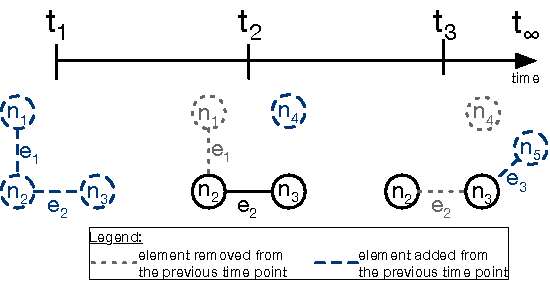
\includegraphics{img/chapt-tkm/formalism/validityExample}
	\caption{Evolution of a temporal graph over time}
	\label{fig:tkm:validityEx}
\end{figure}

In order to augment the graph with a temporal dimension, the relation $V^T$ is added.
So now the knowledge $K$ is defined as a temporal graph such as $K = (N, E, V^T)$.

A node is considered valid either until it is removed or until one of its attributes value changes. 
In the latter case, a new node with the updated value is created.
Whilst, an edge is considered valid until either its source node and target node are valid, or until the edge itself is removed.
Otherwise, nodes and edges are considered invalid.
The temporal validity relation is defined as $V^T: N \cup E \rightarrow I$.
It takes as a parameter a node or an edge ($k \in N \cup E$) and returns a time interval ($i \in I$, \cf Section~\ref{sec:tkm:timeDef}) during which the graph element is valid.

Figure~\ref{fig:tkm:validityEx} shows an example of a temporal graph $K_1$ with five nodes ($n_1$, $n_2$,$n_3$, $n_4$, and $n_5$) and three edges ($e_1$, $e_2$, and  $e_3$) over a lifecycle from $t_1$ to $t_3$.
In this way, $K_1$ equals $(\{n_1, n_2, n_3, n_4, n_5\}, \{e_1, e_2, e_3\}, V^{T}_1)$.
Let's assume that the graph is created at $t_1$.
As $n_1$ is modified at $t_2$, its validity period starts at $t_1$ and ends at $t_2$: $V^{T}_1(n_1) = [t_1, t_2)$.
$n_2$ and $n_3$ are not modified; their validity period thus starts at $t_1$ and ends at $t_\infty$: $V^{T}_1(n_2) = V^{T}_1(n_3) = [t_1, t_\infty)$.
Regarding the edges, the first one, $e_1$, is between $n_1$ and $n_2$ and the second one, $e_2$ from $n_2$ to $n_3$.
Both are created at $t_1$.
As $n_1$ is being modified at $t_2$, its validity period goes from $t_1$ to $t_2$:  $V^{T}_1(e_1) = [t_1, t_2)$.
$e_2$ is deleted at $t_3$.
Its validity period is thus equal to: $V^{T}_1(e_2) = [t_1, t_3)$.

\paragraph{Lifecycle of a knowledge element}
One node represents the state of exactly one knowledge element during a period named the validity period.
The lifecycle of a knowledge element is thus modeled by a unique set of nodes.
By definition, the validity periods of different nodes cannot overlap.
A same time period cannot be represented by two different nodes, which could create inconsistency in the temporal graph.

To keep track of this knowledge element history, the $Z^T$ relation is added to the graph formalism: $K = (N, E, V^T, Z^T)$.
It serves to trace the updates of a given knowledge element at any point in time. 
This relation can also be seen as a temporal identity function which takes as parameters a given node $n \in N$ and a specific time point $t \in T$, and returns the corresponding node at that point. 
Formally, $Z^T: N \times T \rightarrow N$. 

In order to consider this new relation in the example presented in Figure~\ref{fig:tkm:validityEx}, the definition of $K_1$ is modified to $K_1 = (\{n_1, n_2, n_3, n_4, n_5\}, \{e_1, e_2, e_3\}, V^{T}_1, Z^{T}_1)$
In Figure~\ref{fig:tkm:validityEx}, let's imagine that $n_1$, $n_4$, and $n_5$ represent the same knowledge element $k_e$.
The lifecycle of $k_e$ is thus:
\begin{itemize}
    \item $n_1$ for period $[t_1, t_2)$,
    \item $n_4$ for period $[t_2, t_3)$,
    \item $n_5$ for period $[t_3, t_\infty)$.
\end{itemize}

Let $t_1'$ be a timepoint between $t_1$ and $t_2$.
When one wants to resolve the node representing the knowledge element at $t_1'$, she or he gets $n_1$ node, no matter of the node input ($n_1$, $n_4$, or $n_5$): $Z^{T}_1(n_4, t_1) = n_1$.
On the other hand, applying the same relation with another node ($n_2$ or $n_3$) returns another node.
For example, if $n_2$ and $n_3$ do not belong to the same knowledge element, then it will return the node given as input, for example $Z^{T}_1(n_2, t_1) = n_2$.

\paragraph{Knowledge elements stored in nodes}
Nodes are used to store the different knowledge elements: context, requirements and actions.
The set of nodes $N$ is thus split in three subsets: $N = C \cup R \cup A$ where $C$ is the set of nodes which store context information, $R$ a set of nodes for requirement information and $A$ a set of nodes for action information.

Actions define processes that indirectly impact the context: they will change the behaviour of the system, which will be reflected in the context information.
Requirements are also processes that are continuously run over the system in order to check the specifications.
Here, the purpose of the $A$ and $R$ subset is not to store these processes but to list them.
It can be thought as a catalogue of actions and requirements, with their history.

Using a high-level overview, these processes can be depicted as: taking the knowledge as input, perform tasks, and modify this knowledge as output.
As detailed in the next two paragraphs, action executions and requirement analysis can be formalized by relations.

\paragraph{Temporal queries for requirements}
At the current state, the formalism of the knowledge $K$ does not contain any information regarding the requirement analysis.
To overcome this, system requirements analysis $R_A$ are added such as $K = (N, E, V^T, Z^T, R_A)$.
$R_A$ is a set of couples composed of patterns $P_{[t_j,t_k]}(K)$ and requirements $R$ over these patterns: $R_P = {P \cup R}$. 

$P_{[t_j, t_k]}$ denotes a temporal graph pattern, where $t_j$ and $t_k$ are the lower and upper bound of the time interval respectively.
$P_{[t_j, t_k]}$ is the result of a function which takes the knowledge and an interval as input: $P_{[t_j, t_k]} : K \times I$.
The time interval can be either fixed (absolute), \ie both bounds are precisely defined, or sliding (relative), \ie the upper bound is computed from the lower bound.
For example, $P_{[t_0, t_4]}$ is considered as fixed and $P_{[t_0, t_0+4]}$ is considered as relative.
Each element of the pattern should be valid for at least one timepoint: $\forall~p \in P_{[t_j,t_k)}, V^T(e) \cap [t_j,t_k) \neq \emptyset$.
Patterns can be seen as temporal subgraphs of $K$, with a time limiting constraint coming in the form of a time interval.

\paragraph{Temporal relations for actions}
Like for $R_A$, the knowledge $K$ needs to be augmented with action executions $A_E$: $K = (N, E, V^T, Z^T, R_A, A_E)$.
Actions executions $A_E$ can be regarded as a couple $(A, A_F)$, where $A$ is the action that is executed and $A_F$ a set of relations or isomorphisms mapping a source temporal graph pattern $P_{[t_j, t_k]}$ to a target one $P_{[t_l, t_m]}$,  $A_F : K \times I \rightarrow K \times I$.

The left-hand side of the $A_F$ relation depicts the temporal graph elements over which an action is applied.
Every relation may have a set of application conditions. 
They describe the circumstances under which an action should take place. 
These application conditions are either positive, should hold, or negative, should not hold. 
Application conditions come in the form of temporal graph invariants.  
The side effects of these actions are represented by the right-hand side. 

Finally, we associate to $A_E$ a temporal function $E_{A_E}$ to determine the time interval at which an action has been executed. 
Formally, $E_{A_E}: A_E \rightarrow I$.

\paragraph{Temporal relations for decisions}
Finally, the knowledge formalism needs to include the last, but not the least, element: decisions made by the adaptation, $K = (N, E, V^T, Z^T, R_A, A_E, D)$
While the source of relations in $D$ represents the state before the execution of an action, the target shows its impact on the \gls{context}. 
Its intent is \textbf{to trace back impacts of action executions to the decisions they originated from}.  

A decision present in ${D}$ is defined as a set of actions executed, \ie a subset of ${A_E}$, combined with a set of requirement analysis, \ie a subset of ${R_A}$.
Formally, ${D} = \{\ {A_D \cup R_D}~|~{A_D}  \subseteq A_E, R_A \subseteq R_P\}$.
We assume that each action should result from only one decision: $\forall a \in {A}, \forall d1, d2 \in {D}~|~a \in d1 \wedge a \in d2 \rightarrow d1 = d2$.

The temporal function $E_{A_E}$ is extended to decisions in order to represent the execution time: $E_{A_E}: (A \cup D) \rightarrow I$.
For decision, the lower bound of the interval corresponds to the lowest bound of the action execution intervals.
Following the same principle, the upper bound of the interval corresponds to the uppermost bound of the action execution intervals.
Formally, $\forall d \in D \rightarrow E_{A_E}(d) = [l,u)$, where $l = \displaystyle \min_{a \in A_d} \{E_{A_E}(a)[start]\}$ and $u = \displaystyle \max_{a \in A_d} \{E_{A_E}(a)[end]\}$.

\paragraph{Sum up}
Knowledge of an adaptive system can be formalism with a temporal graph such as $K = (N, E, V^T, Z^T, R_A, A_E, D)$, wherein:
\begin{itemize}
    \item $N$ is a set of nodes to represent the different information (context, actions and requirements)
    \item $E$ is a set of edges which connects the different nodes,
    \item $V^T$ is a temporal relation which defines the temporal validity of each element,
    \item $Z^T$ is a relation to track the history of each knowledge elements,
    \item $R_A$ is a relation that defines the different requirements processes,
    \item $A_E$ is a relation that defines the different action processes,
    \item $D$ is a set of action executions, which result from the same decision, and requirement analysis.
\end{itemize}

Decisions $D$ can allow adaptation processes to reason over ongoing and future executions of decisions.
Moreover, it allows tracing the state of the knowledge before and after the decision has been or is executed, thanks to its $A_D$ component.
Plus, it represents which action has been used for this.
Thanks to the $R_A$ relation, one can access the requirements at the root of the decision and the state of the knowledge used by this requirement.

In the next section, we exemplify this formalism over our case study.


\subsection{Application on the use case}

\begin{figure}
	\centering
	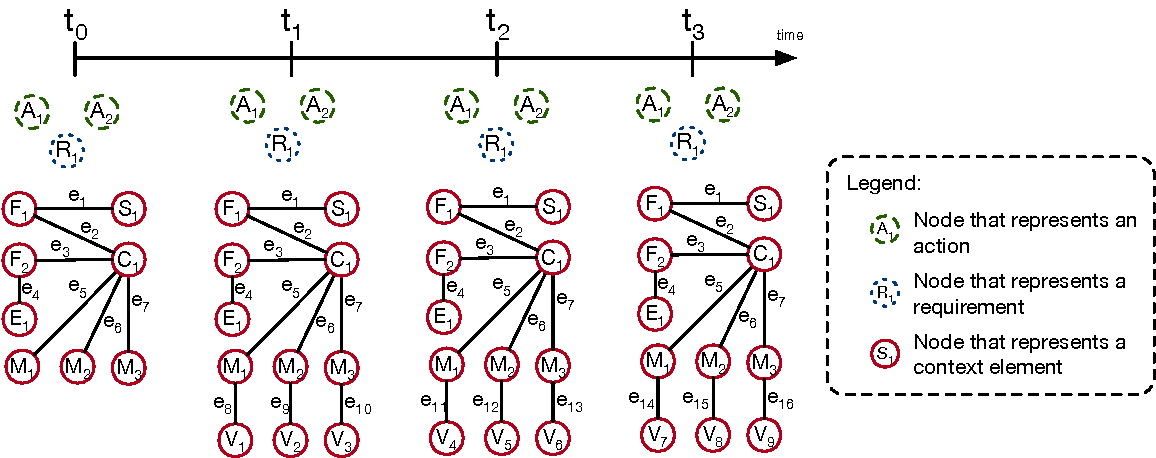
\includegraphics[width=\linewidth]{img/chapt-tkm/formalism/application}
	\caption{Application of the formalism with a temporal graph that represents the knowledge of the smart grid described in Section~\ref{sec:tkm:intro:uc}}
	\label{fig:tkm:k-formalism:application}
\end{figure}

In this section we apply the formalism described on the use case presented in Section~\ref{sec:tkm:intro:uc}.

Let $K_{SG}$ be the temporal graph that represents the knowledge of this adaptive system: $K_{SG} = (N_{SG}, E_{SG}, V^T_{SG}, Z^T_{SG}, R_{P_{SG}}, A_{P_{SG}}, D_{SG})$.
Figure~\ref{fig:tkm:k-formalism:application} shows the nodes and edges of this knowledge.

\paragraph{Description of \pmb{$N_{SG}$}}
$N_{SG}$ is divided into three subsets: $C_{SG}$, $R_{SG}$ and $A_{SG}$.
$R_{SG}$ contains one node, $R_1$ in Figure~\ref{fig:tkm:k-formalism:application}, which represents the requirement of this example (minimizing the number of overloads): $R_{SG} = \{R_1\}$.
Two nodes, $A_1$ and $A_2$, belong to $A_{SG}$: $A_{SG} = \{ A_1, A_2\}$.
They represent the two actions of this example, respectively decreasing and increasing amps limits.
Regarding the context $C_{SG}$, there are three nodes to represent the three smart meters ($M_1$, $M_2$, and $M_3$), one for the substation ($S_1$), two for the fuses ($F_1$ and $F_2$), one for the dead-end cabinet ($E_1$), one for the cable ($C_1$) and one node per consumption value received ($V_i$): $C_{SG} = \{M_1, M_2, M_3, S_1, F_1, F_2, E_1, C_1 \} \cup \{ V_i | i \in [1..9]\}$.

According to the scenario, except for nodes to store consumption values, the other nodes are created at $t_0$ and are never modified.
Therefore, their validity period starts at $t_0$ and never ends: $\forall n \in A_{SG} \cup R_{SG} \cup \{M_1, M_2, M_3, S_1, F_1, F_2, E_1, C_1\}, V^T_{SG}(n) = [t_0, t_\infty)$.
Considering the consumption values, all the nodes represent the history of the values for the three smart meters.
In other words, there are three knowledge elements: the consumption measured for each meter.
Let $C_i$ notes the consumption measured by the smart meter $M_i$.
As shown in Figure~\ref{fig:tkm:contextFormExample}, there is:
\begin{itemize}
	\item $C_1$ of $M_1$ is represented by $\{V_1, V_4, V_7\}$,
	\item $C_2$ of $M_2$ is represented by $\{V_2, V_5, V_8\}$,
	\item $C_3$ of $M_3$ is represented by $\{V_3, V_5, V_9\}$.
\end{itemize}
Taking $C_2$ as an example, $V_2$ is the initial consumption value, replaced by $V_5$ at $t_2$, itself replaced by $V_8$ at $t_3$. 
Applying the $V_{SG}^T$ on these different values, results are thus:
\begin{itemize}
	\item $V_{SG}^T(V_2) = [t_1, t_2)$,
	\item $V_{SG}^T(V_5) = [t_2, t_3)$,
	\item $V_{SG}^T(V_8) = [t_3, t_\infty)$.
\end{itemize}
These validity periods are shown in Figure~\ref{fig:tkm:validityC2}.
As meters send the new consumption values at the same time, this example can also be applied to $C_1$ and $C_3$.

\begin{figure}
	\centering
	\subfloat[Consumption values $C_2$] {
		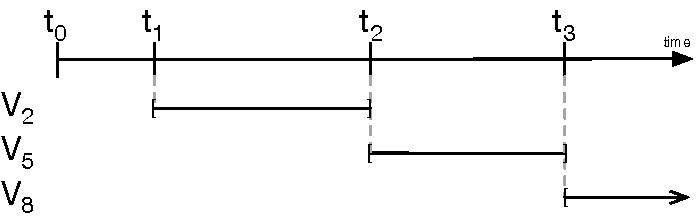
\includegraphics[width=0.4\linewidth]{img/chapt-tkm/formalism/validitySchemaC2}
		\label{fig:tkm:validityC2}
	}
	\hfil
	\subfloat[Edges linking the meter node $M_2$ to its consumption values $C_2$]{
		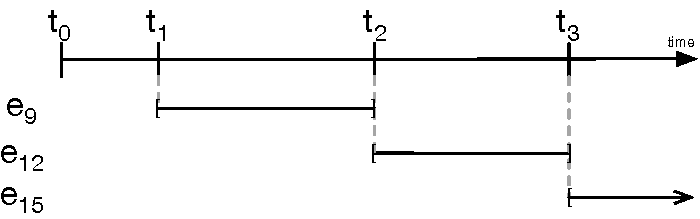
\includegraphics[width=0.4\linewidth]{img/chapt-tkm/formalism/validitySchemaC2Edges}
		\label{fig:tkm:validityC2Edges}
	}
	\caption{Validity periods of consumption values and their edges to the smart meter $M_2$}
\end{figure}

From these validity periods, the $Z^T_{SG}$ can be used to navigate to the different values over time.
Let's continue with the same example, $C_2$.
In order to get the evolution of the consumption value $C_2$, given the initial one, one will use the $Z^T_{SG}$ relation:
\begin{itemize}
	\item $Z^T_{SG}(V_2, t_{s1}) = \emptyset$, where $t_0 \leqslant t_{s1} < t_1$
	\item $Z^T_{SG}(V_2, t_{s2}) = V_2$, where $t_1 \leqslant t_{s2} < t_2$
	\item $Z^T_{SG}(V_2, t_{s3}) = V_5$, where $t_2 \leqslant t_{s3} < t_\infty$.
	\item $Z^T_{SG}(V_2, t_{s4}) = V_8$, where $t_2 \leqslant t_{s4} < t_\infty$.
\end{itemize}


\paragraph{Description of \pmb{$E_{SG}$}}
In this example, edges are used to store the relationships between the different context elements.
For example, the edge between the substation $S_1$ and the fuse $F_1$ allow representing the fact that the fuse is physically inside the substation.
Another example, edges between the cable $C_1$ and the meters $M_1$, $M_2$ and $M_3$ represent the fact that these meters are connected to the smart grid through this cable.

One may consider that relations (validity, $Z^T$, decisions, action executions and requirements analysis) will be stored as edges.
But this decision is let to the implementation part of this formalism.

In our model, only consumption values ($V_i$ nodes) are modified over time.
Plus, since the scenario does not imply any edge modifications, only those between meters and values are modified.
The edge set contains thus sixteen edges: $E_{SG} = \{e_i \mid i \in [1..16] \}$.

By definition, the unmodified edges have a validity period starting from $t_0$ and never ends: $\forall i \in [1..7], V^T_{SG}(e_i) = [t_0, t\infty)$.
The history of the three knowledge elements that represent consumption values do not only impact the nodes which represent the values but also the edges between those nodes and the meters ones:
\begin{itemize}
    \item $C_1$ impacts edges between $M_1$ and $V_1$, $V_4$, and $V_7$, \ie $\{e_8, e_{11}, e_{14}\}$,
    \item $C_2$ impacts edges between $M_2$ and $V_2$, $V_5$, and $V_8$, \ie $\{e_9, e_{12}, e_{15}\}$,
    \item $C_3$ impacts edges between $M_3$ and $V_3$, $V_6$, and $V_9$, \ie $\{e_{10}, e_{13}, e_{16}\}$.
\end{itemize}

Continuing with $C_2$ as an example, the initial edge value is $e_9$ from $t_1$, which is replaced by $e_{12}$ from $t_2$, itself replaced by $e_{15}$ from $t_2$.
The validity relation, applied to these edges, thus returns:
\begin{itemize}
    \item $V^T_{SG}(e_9) = [t_1, t_2) = V^T_{SG}(V_2)$,
    \item $V^T_{SG}(e_{12}) = [t_2, t_3) = V^T_{SG}(V_5)$,
    \item $V^T_{SG}(e_{15}) = [t_3, t_\infty) = V^T_{SG}(V_8)$,
\end{itemize}

These validity periods are depicted in Figure~\ref{fig:tkm:validityC2Edges}.
As they are driven by those of consumption values ($V_2$, $V_5$, and $V_8$), they are equal.

As for nodes, the $Z^T_{SG}$ relation can navigate over time through these values.
For example, to get the history of the edges between the consumption value $C_2$ and the meter represented by $M_2$, one can apply the $Z^T_{SG}$ relation as follows:
\begin{itemize}
    \item $Z^T_{SG}(e_9, t_{s1}) = \emptyset$, where $t_0 \leqslant t_{s1} < t_1$
    \item $Z^T_{SG}(e_9, t_{s2}) = e_9$, where $t_1 \leqslant t_{s2} < t_2$,
    \item $Z^T_{SG}(e_9, t_{s3}) = e_12$, where $t_2 \leqslant t_{s3} < t_3$,
    \item $Z^T_{SG}(e_9, t_{s4}) = e_15$, where $t_3 \leqslant t_{s4} < t_\infty$.
\end{itemize}


\paragraph{Description of \pmb{$D_{SG}$}, \pmb{$A_{E_{SG}}$}, and \pmb{$R_{A_{SG}}$}}
As described in the scenario (cf. Section~\ref{sec:tkm:intro:uc}), the requirement analysis detects that $t_1$ the requirement is broken.
The adaptation process will thus apply the \textquote{decreasing amps limits} action on the three meters.
Following Example 2 detailed in Section~\ref{sec:tkm:intro:motiv:delayed_action}, we consider that the action will impact the consumption values on the next two measurements: $t_2$ and $t_3$. 

In the knowledge, we thus have one decision: $D_{SG} = {D_1}$.
This decision has been taken after one requirement analysis, $R_{A_{SG1}}$, that detects no respect of the requirement $R_1$.
To determine if there is an overload, this analysis needs to know the topology and the consumption values.
The pattern is thus defined by all nodes related to the grid network and consumption values at $t1$: $P_{1[t_1, t_1 + 1]} = \{S_1, F_1, F_2, C_1, E_1, M_1, M_2, M_3, V_1, V_2, V_3\}$.
So we have: $R_{A_{SG1}} = \{ R_1, P_{1[t_1, t_1 + 1]}\}$.

The knowledge also includes the three action executions: $A_{E_{SG1}}$, $A_{E_{SG2}}$, and $A_{E_{SG3}}$.
These actions have been executed on, respectively, $M_1$, $M_2$, and $M_3$.
Following the definition, they all contain the action $A_1$ and similar relation which linked the circumstances to the impacts.
The circumstances are the state of the knowledge at $t_0$, which contain all information of the grid network and the consumption values.
We denote them $P_{2[t_1, t_1 + 1]}$, $P_{3[t_1, t_1 + 1]}$, and $P_{4[t_1, t_1 + 1]}$, all equal $P_{1[t_1, t_1 + 1]}$.
The impact contains all consumption values received at $t_2$ and $t_3$.
Each action impacts the consumption value of the meter that it modifies.
For example, $A_{E_{SG2}}$ only impacts values of meter $M_2$.
For this action, the output pattern is thus : $P_{5[t_2, t_3]} = \{V_5, V_8\}$.
In summary, $A_{E_{SG1}}$, $A_{E_{SG2}}$, and $A_{E_{SG3}}$ are defined as follows: 
\begin{itemize}
    \item for the action executed on $M_1$: $A_{E_{SG1}} = (A_1, A_{F1})$, with $A_{F1}: P_{2[t_1, t_1 + 1]} \rightarrow \{V_4, V_7\}$,
    \item for the action executed on $M_2$: $A_{E_{SG2}} = (A_1, A_{F2})$, with $A_{F2}: P_{3[t_1, t_1 + 1]} \rightarrow \{V_5, V_8\}$,
    \item for the action executed on $M_3$: $A_{E_{SG3}} = (A_1, A_{F3})$, with $A_{F3}: P_{4[t_1, t_1 + 1]} \rightarrow \{V_6, V_9\}$,
\end{itemize}

The decision described in the scenario is thus equal to: $D_1 = \{ R_{A_{SG1}}, A_{E_{SG1}}, A_{E_{SG2}}, A_{E_{SG3}}\}$.
At $t_2$, this decision will still be valid.
The adaptation process can thus include it in the adaptation process to reason over the ongoing actions.
If at $t_3$ the cable remains overloaded, then one may use this element to check if the system tried to fix it, how and based on which information.
 \section{Modelling the knowledge}
\label{sec:tkm:mm}
 
 In order to simplify the diagnosis of adaptive systems, this thesis proposes a novel \gls{metamodel} that combines, what we call, design elements and runtime elements.
Design elements abstract the different elements involved in \gls{knowledge} information to assist the specification of the adaptation process.
Runtime elements instead, represent the data collected by the adaptation process during its execution.
In order to maintain the consistency between previous design elements and newly created ones, instances of design elements (\eg actions) can be either added or removed.
Modifying these elements would consist in removing existing elements and creating new ones.
Combining design elements and runtime elements in the same model helps not only to acquire the evolution of system but also the evolution of its structure and specification (e.g. evolution of the requirements of the system).
Design time elements are depicted in gray in the Figures~\ref{fig:knowledge-mm}--~\ref{fig:action-mm}.
Note that, this thesis does not address how runtime information is collected.

For the sake of modularity, the \gls{metamodel} has been split into four packages: Knowledge, Context, Requirement and Action.
All the classes of these packages have a common parent class that adds the temporality dimension: \textit{TimedElement} class.
Before describing the Knowledge (core) package, we detail this element.
Then, we introduce in more details the other three packages used by the Knowledge package: Context, Requirement, and Action. 
In below sections, we use "\textit{Package::Class}" notation to refer to the provenance of a class.
If the package is omitted, then the provenance package is this one described by the figure or text.

\subsection{Parent element: \textit{TimedElement} class}
We assume that all the classes in the different packages extend a \textit{TimedElement} class. 
This class contains three methods: \textit{startTime}, \textit{endTime}, and \textit{modificationsTime}.
The first two methods allow accessing the validity interval bounds defined by the previously discussed $V^T$ relation.
The last method resolves all the timestamps at which an element has been modified: its history. 
This method is the implementation of the relation $Z^T$ described in our formalism (cf. Section~\ref{sec:tkm:k-formalism:formalism}).


\subsection{Knowledge metamodel}
\label{sec:tkm:mm:knoeldge}

\begin{figure*}[t]
	\centering
	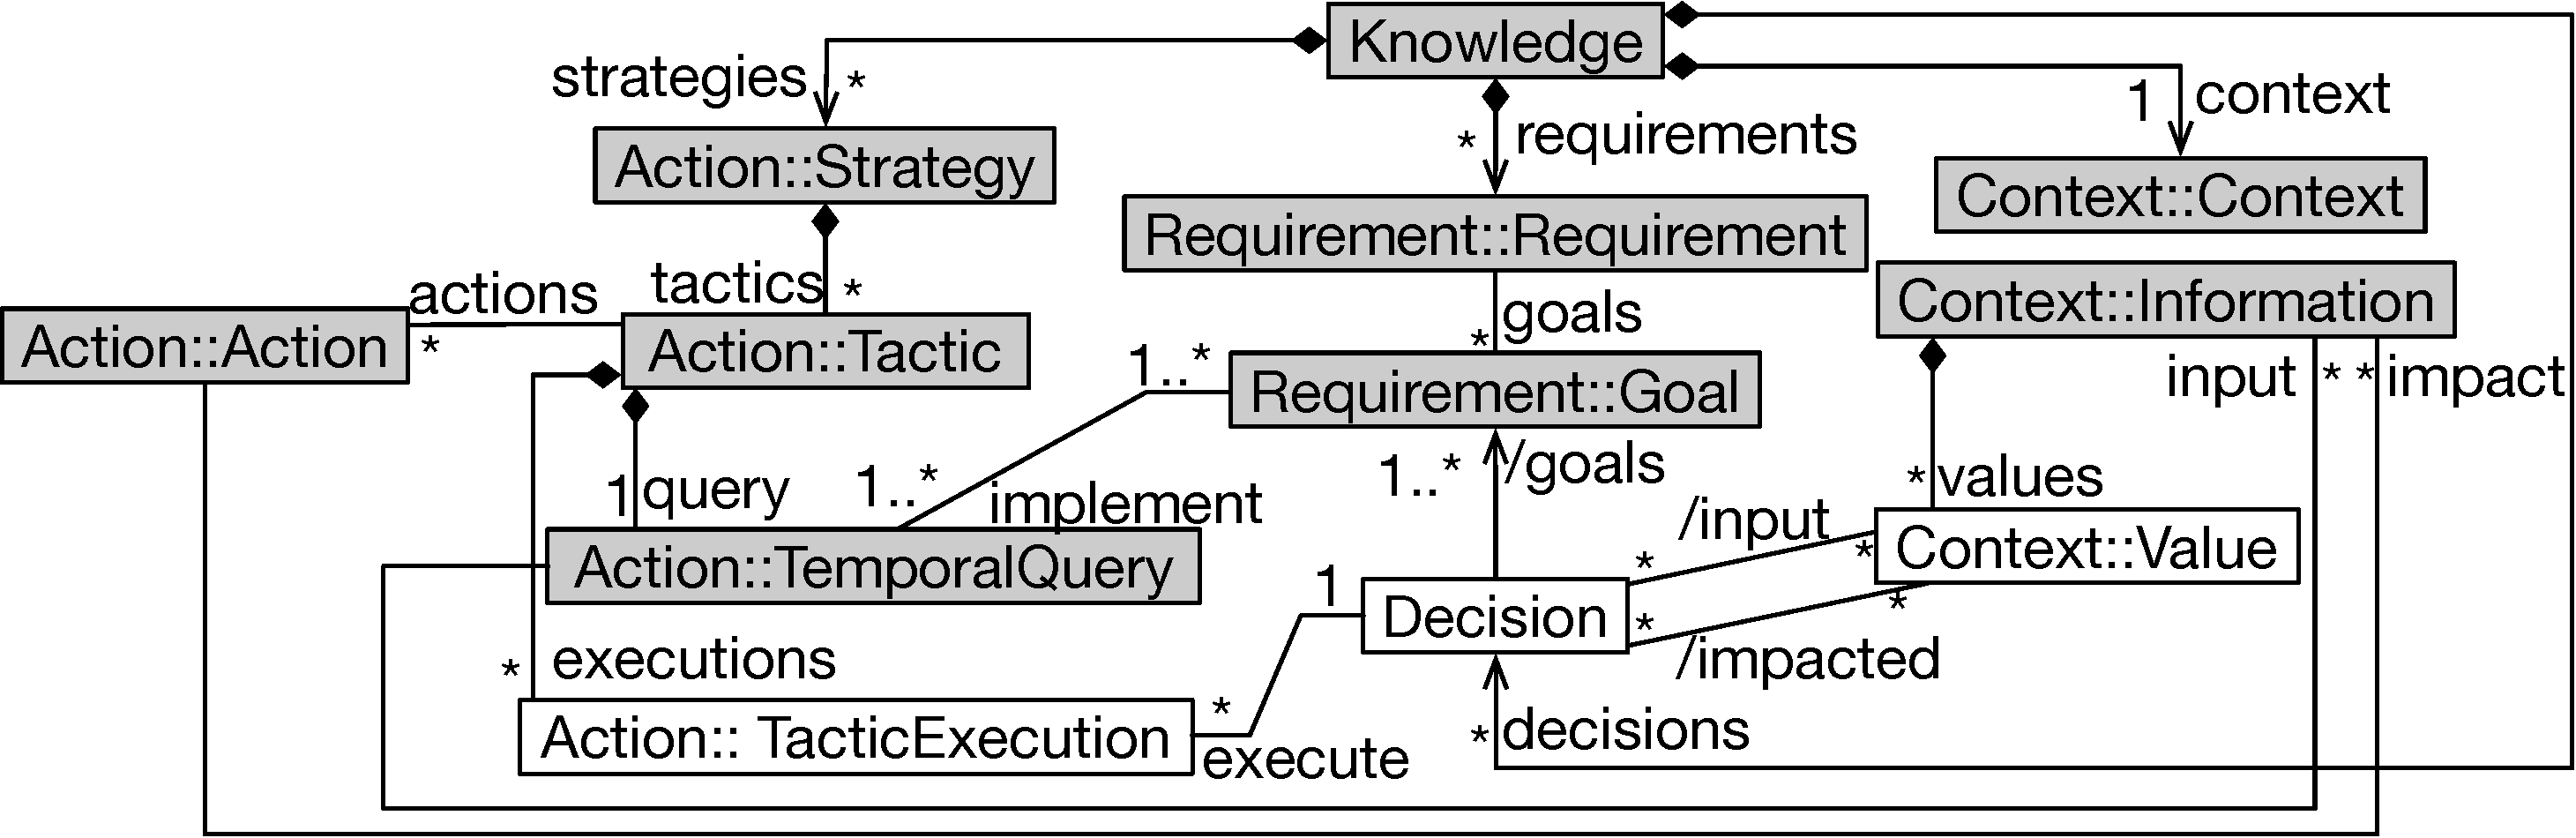
\includegraphics[width=.9\linewidth]{img/chapt-tkm/mm/knowledge-mm}
	\caption{Excerpt of the knowledge metamodel}
	\label{fig:knowledge-mm} 
\end{figure*}

In order to enable interactive diagnosis of adaptive systems, traceability links between the decisions made and their circumstances should be organized in a well-\linebreak structured representation. 
In what follows, we introduce how the \gls{knowledge} \gls{metamodel} helps to describe \glspl{decision}, which are linked to their  goals and their context (input and impact). 
Figure~\ref{fig:knowledge-mm} depicts this \gls{metamodel}.

Knowledge package is composed of a \textit{\gls{context}}, a set of \textit{\glspl{requirement}}, a set of \textit{strategies}, and a set of \textit{\glspl{decision}}.
A \gls{decision} can be seen as the output of the Analyze and Plan steps in the \gls{mapek} loop.

Decisions comprise target \textit{goals} and trigger the execution of one \textit{tactic} or more.  
A decision has an \textit{input} context and an \textit{impacted} context.
The context impacted by a decision  (\textit{Decision.impacted}) is a derived relationship computed by aggregating the impacts of all actions belonging to a decision (see Fig.~\ref{fig:action-mm}).
Likewise, the \textit{input} relationship is derived and can be computed similarly. 
In the smart grid example, a decision can be formulated (in plain English) as follows: since the district D is almost overloaded (\textit{input context}), we reduce the amps limit of greedy consumers using the ``\textit{reduce amps limit}" \textit{action} in order to reduce the load on the cable of the district (\textit{impact}) and satisfy the ``\textit{no overload}" policy (\textit{requirement}).

As all the elements inherit from the \textit{TimedElement}, we can capture the time at which a given decision and its subsequent actions were executed, and when their impact materialized, \ie measured.
Thanks to this metamodel representation, a developer can apprehend the possible causes behind malicious behaviours by navigating from the context values to the decisions that have impacted its value (\textit{Property.expected.impact}) and the goals it was trying to reach (\textit{Decision.goals}).
An example for such in interactive diagnosis can be found in Section~\ref{sec:tkm:intro:uc}.

\subsection{Context metamodel}
\begin{figure*}
 	 \centering
      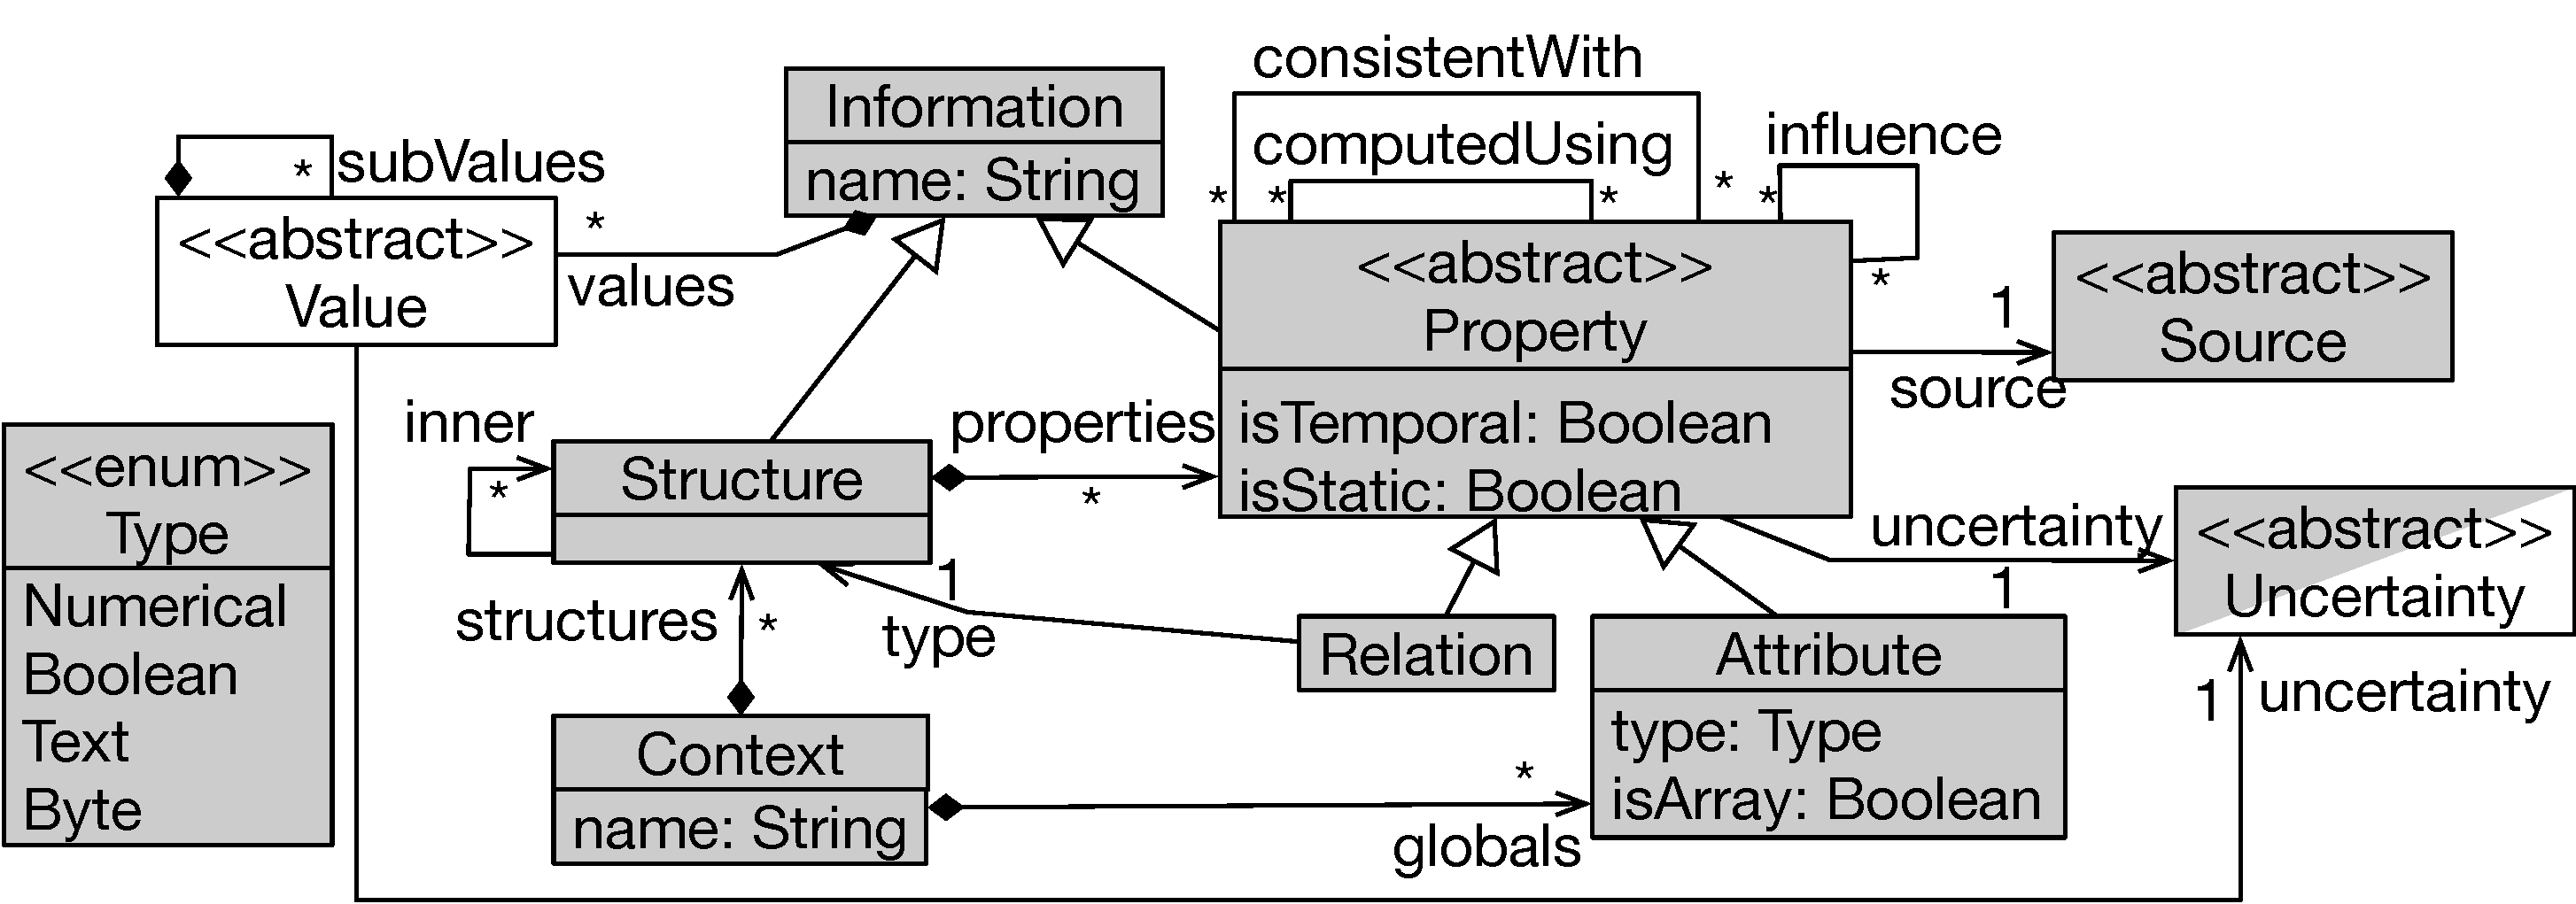
\includegraphics[width=.8\linewidth]{img/chapt-tkm/mm/contextModel}
      \caption{Excerpt of the context metamodel}
      \label{fig:context-model}
\end{figure*}

Context models structure context information acquired at runtime. 
For example, in a smart-grid system, the context model would contain information about smart-grid users (address, names, etc.) resource consumption, etc.

An excerpt of the context model is depicted in Figure~\ref{fig:context-model}. 
we propose to represent the context as a set of structures (\textit{Context.structures}) and global attributes (\textit{Context.globals}).
A structure can be viewed as a C-structure with a set of properties (\textit{Property}): attributes (\textit{Attribute}) or relationships (\textit{Relation}).
A structure may contain other nested structures (\textit{Structure.inner}).
Structures and properties have values.
They correspond to the nodes described in the formalization section (\cf Section~\ref{sec:tkm:k-formalism:formalism}).
The connection feature described in Section~\ref{sec:back:adapt:knowledge:req} is represented thanks to three recursive relationships on the Property class: \textit{consistentWith}, \textit{computedUsing} and \textit{influence}.
Additionally, each property has a source (\textit{Source}) and an uncertainty (\textit{Uncertainty}).
It is up to the stakeholder to extend data with the appropriate source: measured, computed, provided by a user, or by another system (\eg weather information coming from a public API).
Similarly, the uncertainty class can be extended to represent the different kinds of uncertainties. Finally, a property can be either historic or static.

\subsection{Requirement metamodel}

\begin{figure}
	\centering
	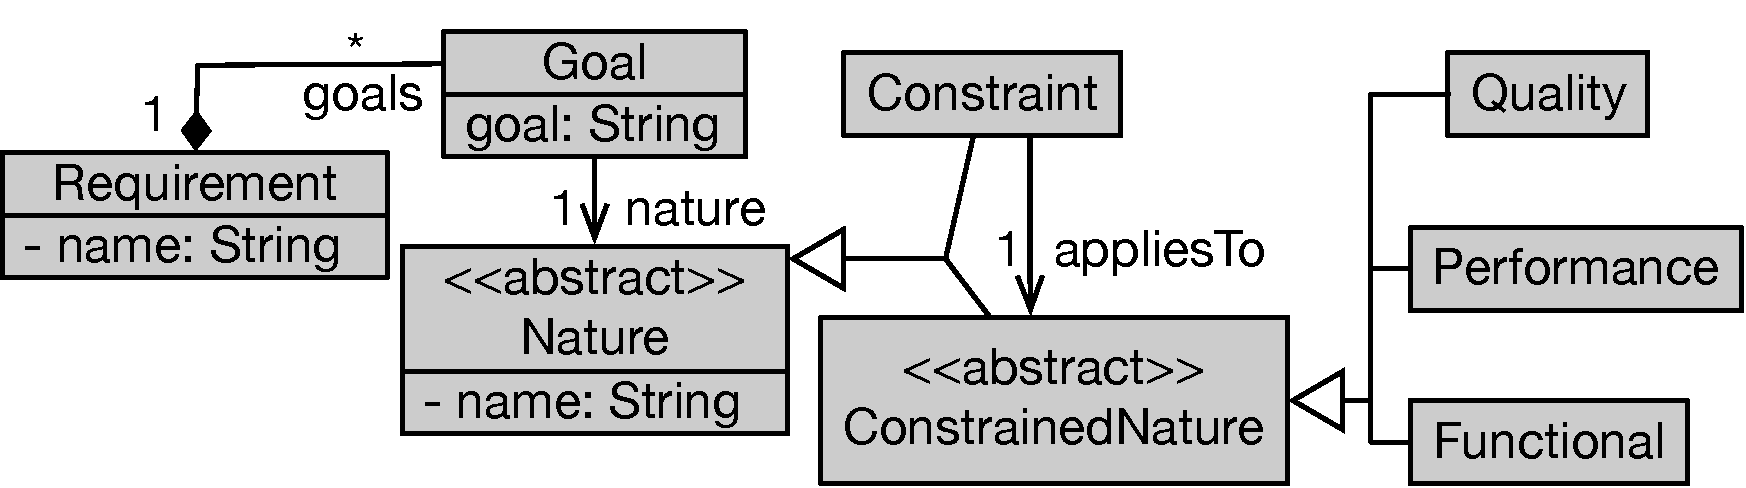
\includegraphics[width=0.7\linewidth]{img/chapt-tkm/mm/requirementModel}
	\caption{Requirement metamodel}
	\label{fig:requirement-model}
\end{figure}

As different solutions to model system requirements exist (\eg KAOS~\cite{DBLP:journals/scp/DardenneLF93}, i*~\cite{yu2011modelling} or Tropos~\cite{DBLP:journals/aamas/BrescianiPGGM04}), in this metamodel, we abstract their shared concepts.
The requirement model, depicted in Figure~\ref{fig:requirement-model}, represents the \textit{requirement} as a set of \textit{goals}.
Each goal has a \textit{nature} and a textual specification.
The nature of the goals adheres to the four categories of requirements presented in Section~\ref{sec:back:adapt:knowledge:req}.
One may use one of the existing requirements modelling languages (\eg RELAX) to define the semantics of the requirements. 
Since the requirement model is composed solely of design elements, we may rely on static analysis techniques to infer the requirement model from existing specifications.
The work of Egyed~\cite{DBLP:conf/icse/Egyed01} is one solution among others.
This work is out of the scope of the thesis and envisaged for future work. 

In the guidance example, the requirement model may contain a \textbf{balanced resource distribution} requirement.
It can be split into different goals: (i) \textit{minimizing overloads}, (ii) \textit{minimizing production lack}, (iii) \textit{minimizing production loss}.

\subsection{Action metamodel}

\begin{figure}
	\centering
	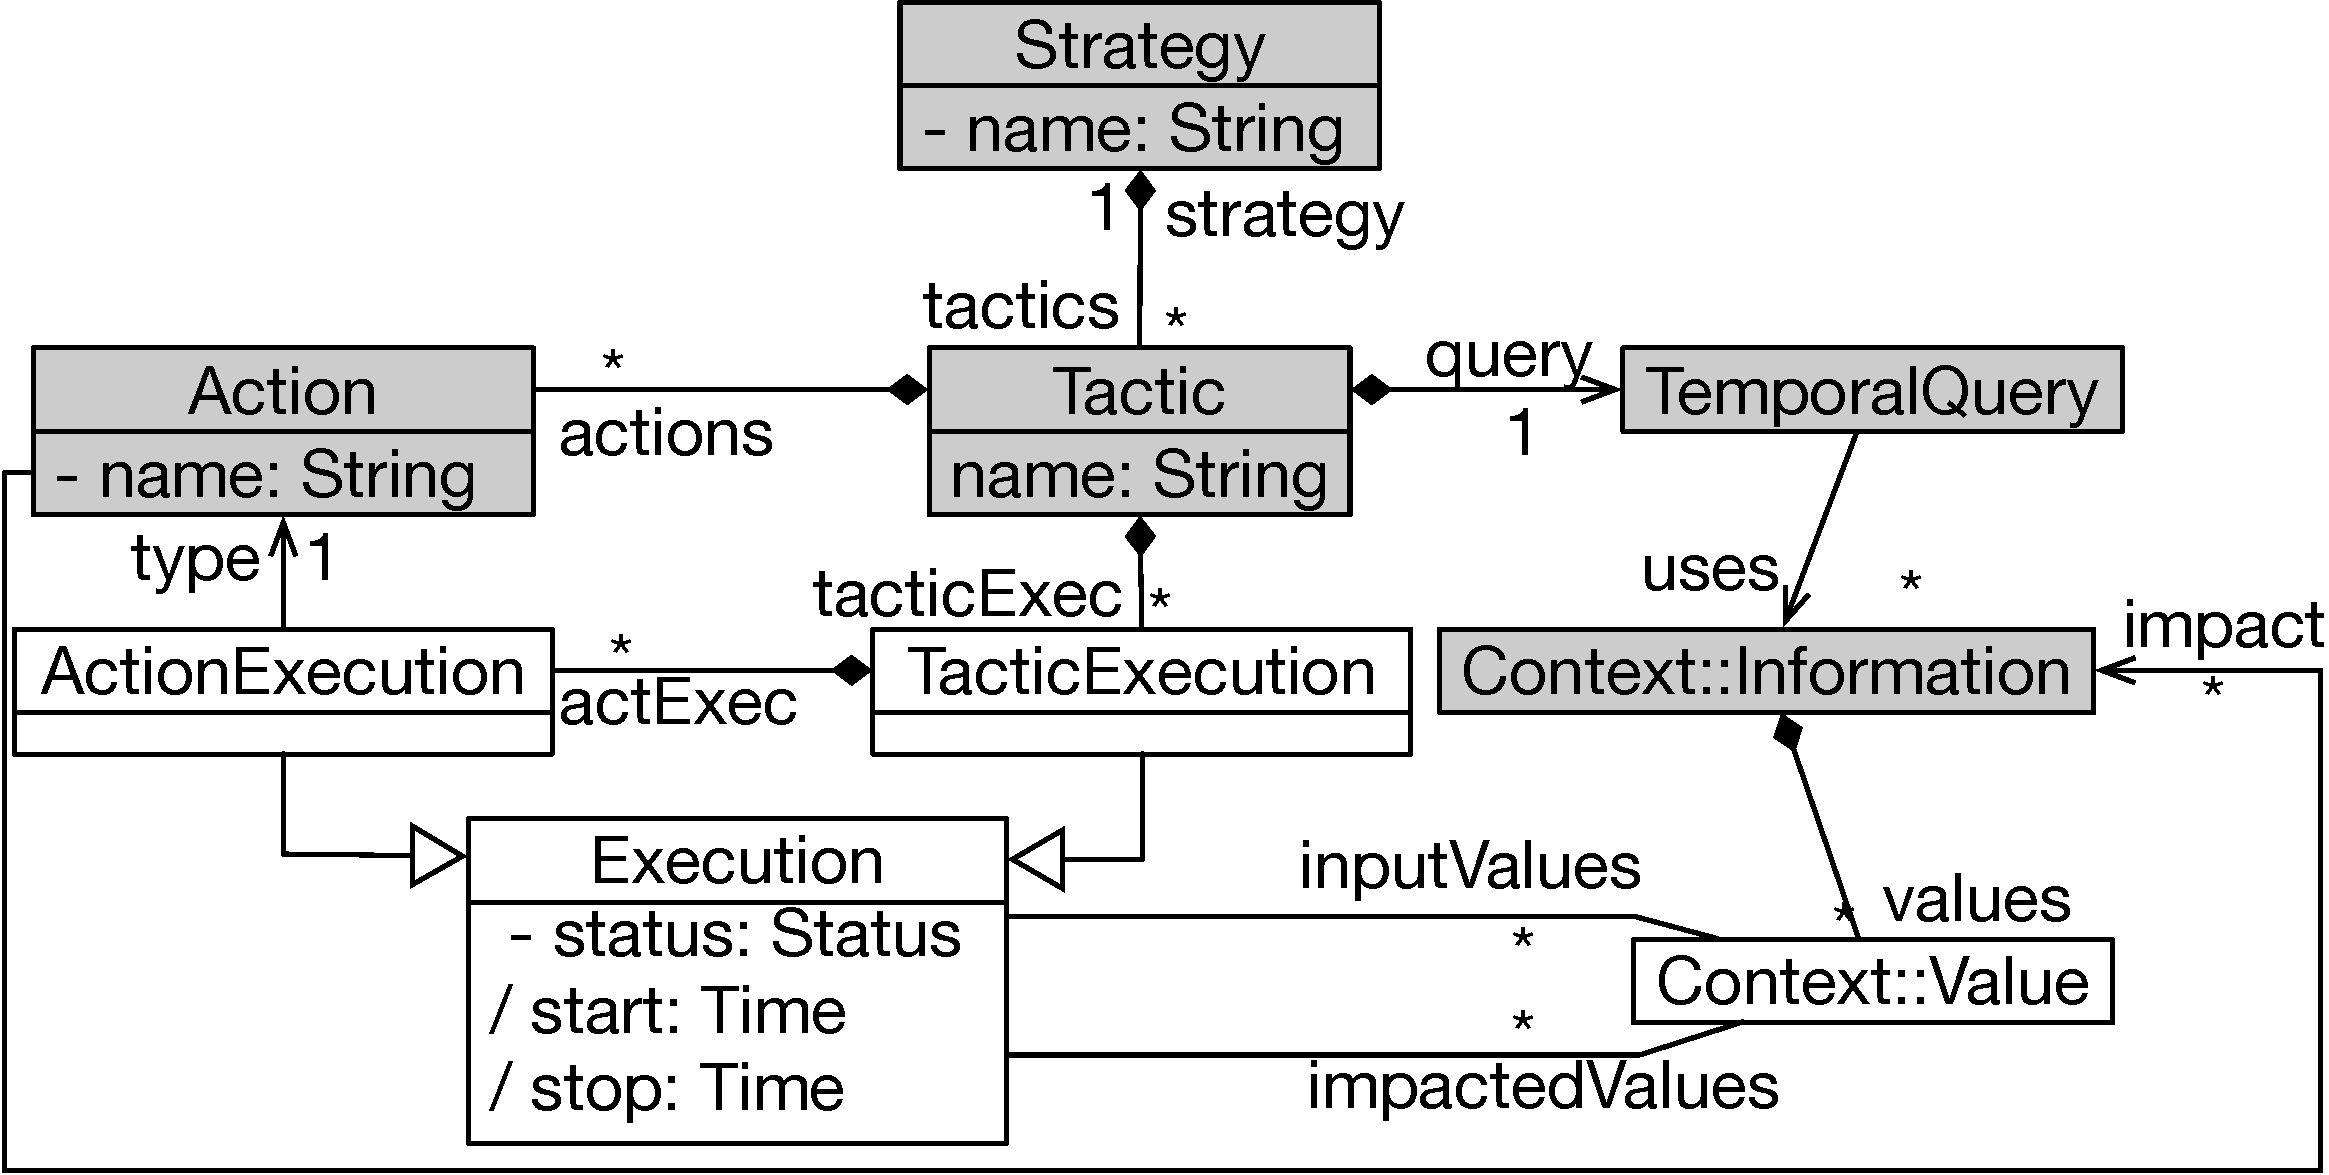
\includegraphics[width=0.8\linewidth]{img/chapt-tkm/mm/actionModel}
	\caption{Excerpt of the action metamodel}
	\label{fig:action-mm}
\end{figure}

Similar to the requirements metamodel, the actions metamodel also abstracts main concepts shared among existing solutions to describe adaptation processes and how they are linked to the context. 
Figure~\ref{fig:action-mm} depicts an excerpt of the action metamodel.
we define a strategy as a set of tactics (\textit{Strategy}).
A tactic contains a set of actions (\textit{Action}).
A tactic is executed under a precondition represented as a temporal query (\textit{TemporalQuery}) and uses different data from the context as input.
In future work, we will investigate the use of preconditions to schedule the executions order of the actions, similarly to existing formalisms such as Stitch~\cite{DBLP:journals/jss/ChengG12}.
The query can be as complex as needed and can navigate through the whole knowledge model.
Actions have impacts on certain properties, represented by the \textit{impacted} reference. 

The different executions are represented thanks to the \textit{Execution} class. Each execution has a status to track its progress and links to the impacted context values(\textit{Execution.impactedValues}).
Similarly, input values are represented thanks to the \textit{Execution.inputValues} relationship.
An execution has \textit{start} and \textit{end} time. Not to confuse with the \textit{startTime} and \textit{endTime} of the validity relation $V^T$.
Whilst the former corresponds to the time range in which a value is valid, the \textit{start} and \textit{stop} time in the class execution correspond to the time range in which an action or a tactic was being executed.
The start and stop attributes correspond to the relationL $E_{A_E}$ (see Section~\ref{sec:tkm:k-formalism:formalism}). These values can be derived based on the validity relation.
They correspond to the time range in which the status of the execution is \textquote{\textit{RUNNING}}.
Formally, for every execution node $e$, $E_{A_E}(e)~=~(V(e)~|~e.status~=~$\textquote{RUNNING}$)$.


Similarly to requirement models, it is possible to automatically infer design elements of action models by statically analyzing actions specification.
Since acquiring information about tactics and actions executions happens at runtime, one way to achieve this is by intercepting calls to actions executions and updating the appropriate action model elements accordingly.
This is out of the scope of this thesis and planned for future work.
 \section{Validation}
\label{sec:tkm:validation}

To validate and evaluate our approach, we implemented a prototype publicly available online\footnote{https://github.com/lmouline/LDAS}.
This implementation leverages the GreyCat framework\footnote{https://github.com/datathings/greycat}, more precisely the modeling plugin, which allows designing a metamodel using a textual syntax.
Based on this specification, GreyCat generates a Java and a JavaScript API to create and manipulate models that conform to the predefined metamodel.
The GreyCat framework handles time as a built-in concept.
Additionally, it has a native support of a lazy loading mechanism and an advanced garbage collection.
This is achieved by dynamically loading and unloading model elements from the main memory when necessary.

The validation of our approach has been driven by the two research questions formulated in the introduction section:
\begin{itemize}
	\item How to diagnose the self-adaptation process?
	\item How to enable reasoning over unfinished actions and their expected effects?
\end{itemize}

To address the first one, we describe how one can use our approach to represent the knowledge an adaptation process for a smart grid system.
Then, we present a code to extract the circumstances and the goals of a decision.
For the second one, we present a scenario where a developer can use our approach to reason over unfinished actions and their expected effects.
The presented code shows how information can be extracted from our model to enable any reasoning algorithm.
Finally, we present performance evaluation to show the scalability of our approach.

\subsection{Diagnostic: implementation of the use case}
In what follows, we explain how a stakeholder, Morgan, can apply our approach to a smart grid system in order to, first, abstract adaptive system concepts, then, structure runtime data, and finally, query the model for diagnosis purpose.
The corresponding object model is depicted in Figure~\ref{fig:tkm:valid:diag}.
Due to space limitation, we only present an excerpt of the knowledge model.
An elaborate version is accessible in the tool repository.\looseness=-1

\paragraph{Abstracting the adaptive system}

At design time ($t_d$), either manually or using an automatic process, Morgan abstracts the different tactics and actions available in the adaptation process.
Among the different tactics that Morgan would like to model is  ``\textit{reduce amps limit}". 
It is composed of three actions: sending a request to the smart meter (\textit{askReduce}), checking if the new limit corresponds to the desired one (\textit{checkNewLimit}), and notifying the user by e-mail (\textit{notifyUser}). 
Morgan assumes that the \textit{askReduce} action impacts consumption data (\textit{csmpt}).
This tactic is triggered upon a query (\textit{tempQ}) that uses meter (\textit{mt}), consumption (\textit{csmpt}) and customer (\textit{cust}) data. The query implements the ``\textit{no overload}" goal: the system shall never have a cable overload. 
Figure~\ref{fig:tkm:valid:diag} depicts a flattened version of the temporal model representing these elements. The tag at upper-left corner of every object illustrates the creation timestamp. All the elements created at this stage are tagged with $t_d$.

\paragraph{Adding runtime information}
The adaptation process checks if the current system state fulfills the requirements by analyzing the context. To perform this, it executes the different temporal queries, including \textit{tempQ}.
For some reasons, the {tempQ} reveals that the current context does not respect the ``\textit{no overload}" goal. To adapt the smart grid system, the adaptation process decides to start the execution of the previously described tactic (\textit{exec1}) at $t_s$. As a result,  
a decision element is added to the model along with a relationship to the unsatisfied goal. In addition, this decision entails the planning of a tactic execution, manifested in the creation of the element \textit{exec1}and its subsequent actions (\textit{notifyU}, \textit{checkLmt}, and \textit{askRed}). At $t_s$, all the actions execution have an IDLE status and an expected start time. All the elements created at this stage are tagged with the $t_s$ timestamp in Figure~\ref{fig:tkm:valid:diag}.\looseness-1

At $t_{s+1}$, the planned tactic starts being executed by running the action \textit{askReduce}. The status of this action turns from \textit{IDLE} to \textit{RUNNING}. Later, at $t_{s+2}$, the execution of \textit{askReduce} finishes with a \textit{SUCCEED} status and triggers the execution of the actions \textit{notifyUser} and \textit{checkNewLimit} in parallel. The status of \textit{askReduce} changes to \textit{SUCCEED} while the status of \textit{notifyUser} and \textit{checkNewLimit} turns to \textit{RUNNING}.
The first action successfully ends at $t_{s+3}$ while the second ends at $t_{s+4}$. As all actions terminates with a \textit{SUCCEED} status at $t_{s+4}$, accordingly, the final status of the tactic is set \textit{SUCCEED} and the \textit{stop} attribute value is set to $t_{e}$.  

\begin{figure}
	\centering
	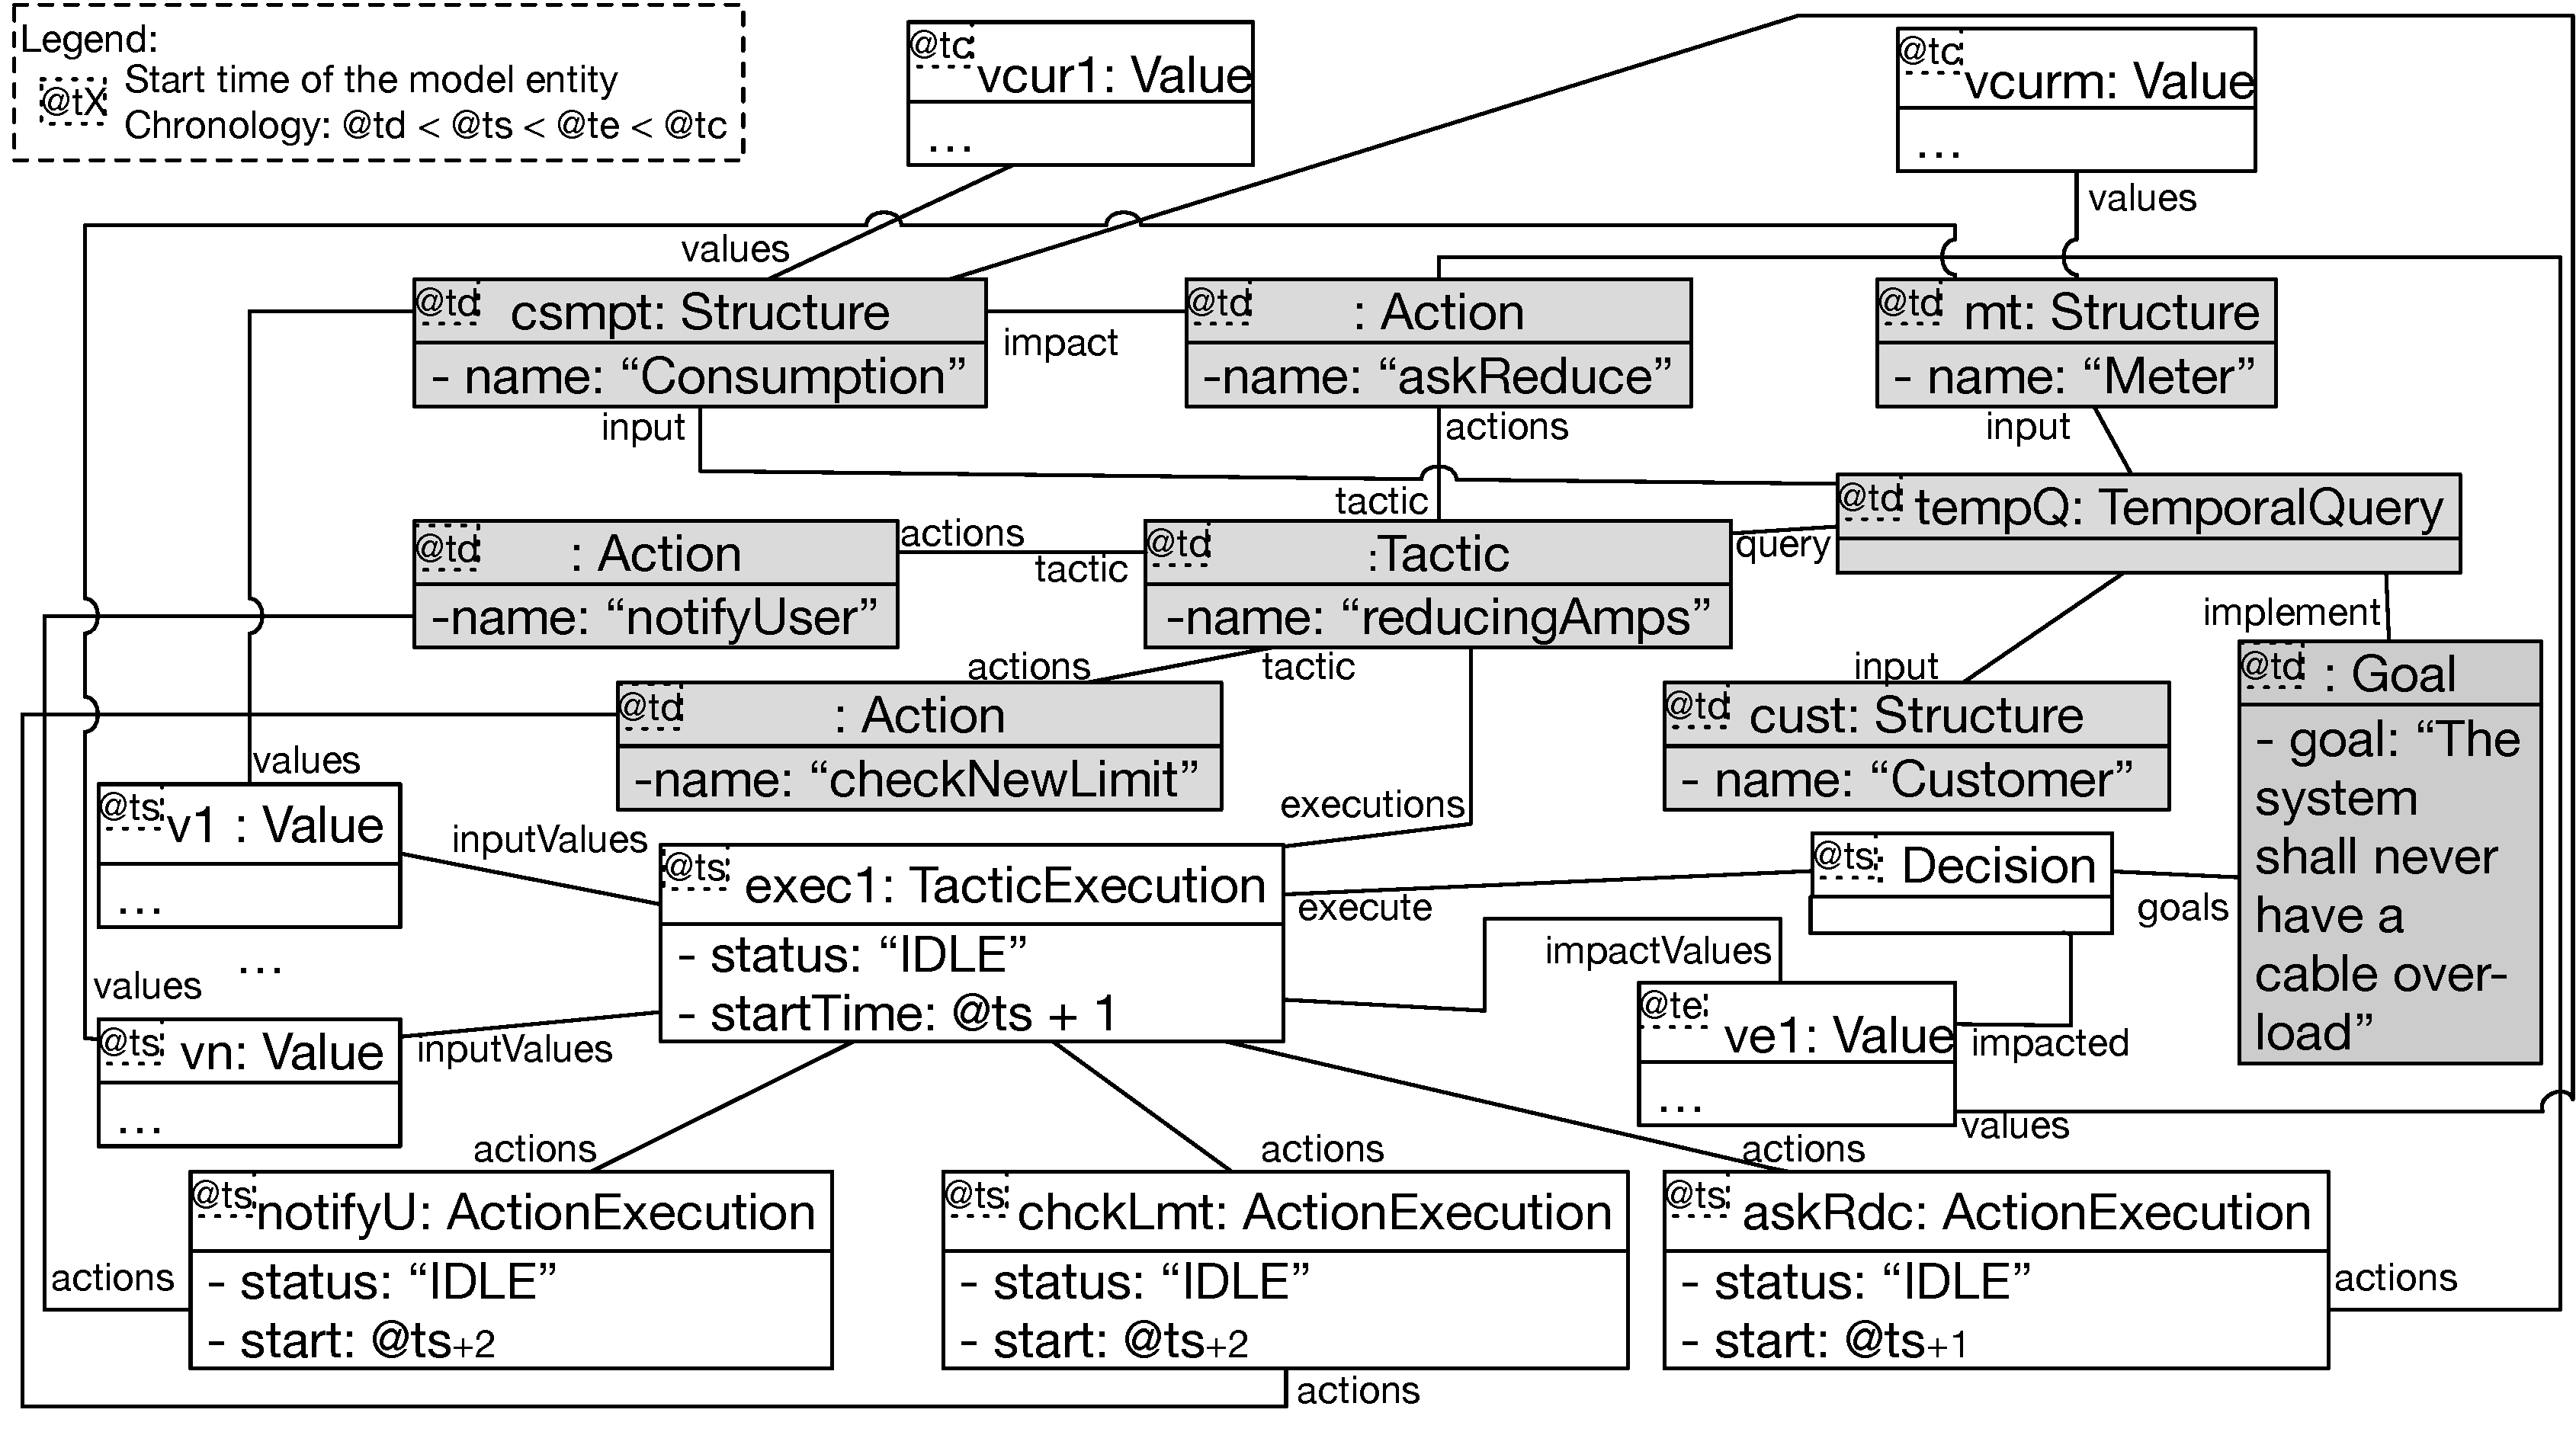
\includegraphics[width=\linewidth]{img/chapt-tkm/validation/action-om}
	\caption{Excerpt of the knowledge object model related to our smart grid example}
	\label{fig:tkm:valid:diag}
\end{figure}

\paragraph{Interactive diagnosis query}
After receiving incident reports concerning regular power cuts, and based on the aforementioned knowledge model, Morgan would be able to query the system's states and investigate why such incidents have occurred.
As described in Section~\ref{sec:example}, she/he will interactively diagnose the system by interrogating the context, the decisions made, and their circumstances.

The first function, depicted in Listing~\ref{code:actions-to-goals}, allows  to navigate from the currently measured values (\textit{vcur1}) to the decision(s) made. The for-loop and the if-condition are responsible for resolving the measured data for the past two days. 
Past elements are accessed using the \textit{resolve} function that implements the $\mathcal{Z}^T$ relation (\cf Section~\ref{sec:formalism}).
After extracting the decisions leading to power cuts, Morgan carries on with the diagnosis by accessing the circumstances of this decision. The code to perform this task is depicted in Listing~\ref{code:actions-to-goals}, the second function (getCircumstances).
Note that the relationship \textit{Decision.input} is the aggregation of \textit{Decision.excecute.inputValues}.

\begin{lstlisting}[style=customc,caption=Get the goals used by the adaptation process from executed actions, label=code:actions-to-goals,basicstyle=\scriptsize]
// extracting the decisions
Decision[] impactedBy(Value v) {
  Decision[] respD
  for( Time t: v.modificationTimes() ):
    if (t >= v.startTime() - 2 day)
      Value resV = resolve(v,t)
    respD.addAll(from(resV).navigate(Value.impacted))
  return respD
}
// extracting the circumstances of the made decisions
Tuple<Value[], Goal[]> getCircumstance(Decision d) {
  Value[] resValues = from(d).navigate(Decision.input)
  Goal[] resGoals = from(d).navigate(Decision.goals)      
  return Tuple<>(resValues, resGoals)
} 
\end{lstlisting}

\subsection{Reasoning over unfinished actions and their expected effects}
By associating the action model to the knowledge model, we aim at enhancing adaptation process with new abilities to reason.
In this section, we present an example of a reasoning algorithm which consider the impacts of running actions.
This example is based on our use case (\cf Section~\ref{sec:intro:use-case}).

Let's imagine that the adaption process detects overloaded cables in the smart grid.
To fix this situation, it takes severals counter measures, among which there are fuse state modifications.
As detailed in Section~\ref{sec:tkm:intro:motiv}, this action is considered as delayed action.
Later, another incident is detected, for example a substation is being overloaded.
Before taking any actions, the adaption process can, thanks to our solution, verify if the running actions will be sufficient to solve this new incidents.
If not, it can either take additional actions or replan the running one.
The algorithm to reschedule current actions or to compute additional actions is out of scope of this thesis.
Here, we present the code to extract required information from our model.

Checking if the running actions will be sufficient to solve all current issues can also be thought as: will the issue remain with the new context, \ie after each actions have been executed.
In our case, it is like verifying if the second overload will still remain with the new topology, which is coming.
The adaptation process therefore needs to extract the context in the future.
To do so, the adaptation process should know the latest timepoint at which the impact will be measured.
Listing~\ref{code:tkm:valid:latest-impact} shows the code to get this timepoint.
Running, idle and finished actions are accessed thanks to the the two first nested loops with the if-condition.
We consider that failed and canceled actions have no effects.
As finished actions may still have effects, we also consider them.
Then we navigate through all impacted values to get their start time, \ie the beginning of their validity period ($V^T$ relation, \cf Section~\ref{sec:tkm:k-formalism:formalism}).
Doing so, we are sure to get the latest timepoint at which an impact will be measurable.

\begin{lstlisting}[style=customc, caption=Get latest timepoint at which the impact will be measured, label=code:tkm:valid:latest-impact,basicstyle=\scriptsize]
Time latestImpact(Knowledge k) {
  Time latestTime = CURRENT_TIME
  
  for(Decision d: from(k).navigate(decisions))
    for(TacticExecution te: from(d).navigate(execute))
      if(te.status == "RUNNING" || te.status == "IDLE" || te.status == "SUCCEED")
        for(Value v: from(te).navigate(impactedValues))
          if(v.startTime() > latestTime)
            latestTime = v.startTime()
            
  return latestTime
}	
\end{lstlisting}

Using this timepoint, then the adaption process can then compute how the grid should be after the actions have been executed.
If the system has no prediction mechanism, then the adaption process can verify how the power will be balance over the new topology.
Otherwise, it can use this prediction feature to compute the expected loads with the coming topology.
Using these information, it can verify if all current incidents will be solved by the ongoing actions or not.
If not, it may take additional actions or reschedule them.

Listing~\ref{code:tkm:valid:extract-act} depicts the code to extract all running actions.
The nested loops allow accessing to all executions made by decision.
Then, we filter only those with the \textquote{RUNNING} status.
The resulting collection should then be given to the scheduling algorithm, which will decide if a rescheduling is possible and how. 

 
\begin{lstlisting}[style=customc, caption=Extract ongoing actions and their effects, label=code:tkm:valid:extract-act,basicstyle=\scriptsize]
TacticExecution[] runningActions(Knowledge k) {
  TacticExecution[] resA
  for(Decision d: k.decisions) {
    for(TacticExecution te: d.execute) {
      if(te.status == Status.RUNNING) {
        resA.add(te)
      }
    }
  }
  return resA
}
\end{lstlisting}

Using our model, developers have to solution to model a rescheduling operation.
Either they modify the actions, which may delete the history of the previous decision, or they mark all running and idle actions as \textquote{CANCELLED} and create a new decision, with new actions, which update the circumstances and re-use the same requirements.

\subsection{Performance evaluation}
GreyCat stores temporal graph elements in several key/value maps. Thus, the complexity of accessing a graph element is linear and depends on the size of the graph. 
Note that in our experimentation we evaluate only the execution performance of diagnosis algorithms. For more information on I/O performance in GreyCat, please refer to the original work by Hartmann \etal~\cite{DBLP:conf/seke/0001FJRT17, DBLP:phd/basesearch/Hartmann16}.

\begin{lstlisting}[style=customc,caption=Traversal used during the experimentations,label=code:traversal-used,basicstyle=\scriptsize]
  MATCH (input)-[*4]->(output)
  WHERE input.id IN [randomly generated set]
  RETURN output
  LIMIT O
\end{lstlisting}

We consider a diagnosis algorithm to be a graph navigation from a set of nodes (input) to another set of nodes (output).
Unlike typical graph algorithms, diagnosis algorithms are simple graph traversals and do not involve complex computations at the node level. Hence, we believe that three parameters can impact their performance (memory and/or CPU): the global size of the graph, the size of the input, and the number of traversed elements.
In our evaluation, we altered these parameters and report on the behavior of the main memory and the execution time. The code of our evaluation is publicly available online\footnote{https://bitbucket.org/ludovicpapers/icac18-eval}.
All experiments reporting on memory consumption were executed 20 times after one warm-up round. Whilst, execution time experiments were run 100 times after 20 warm-up rounds.
The presented results correspond to the mean of all the iterations.
We randomly generate graph with sizes (\textit{N}) ranging from 1\,000 to 2\,000\,000. 
At every execution iteration, we follow these steps: (1) in a graph with size \textit{N}, we randomly select a set of \textit{I} input nodes, (2) then traverse \textit{M} nodes in the graph, (3) and  we collect  the first \textit{O} nodes that are at four hops from the input element. Listing~\ref{code:traversal-used} describes the behavior of the traversal using Cypher, a well-known graph traversal language.

We executed our experimentation on a MacBook Pro with an Intel Core i7 processor (2.6 GHz, 4 cores, 16GB main memory (RAM), macOS High Sierra version 10.13.2). We used the Oracle JDK version 1.8.0\_65.

\paragraph{How performance is influenced by the graph size \textit{N}?}
This experimentation aims at showing the impact of the graph size (\textit{N}) on memory and execution time while performing common diagnosis routines.
We fix the size of \textit{I} to 10. To assure that the behavior of our traversals is the same, we use a seed value to select the starting input elements. We stop the algorithm when we reach 10 elements.
Results are depicted in Figure~\ref{fig:exp1}.

As we can notice, the graph size does not have a significant impact on the execution time of diagnosis algorithms.
For graphs with up to 2,000,000 elements, execution time remains between 2 ms and four 4 ms. We can also notice that the memory consumption insignificantly increases.
Thanks to the implementation of a lazy loading and a garbage collection strategy by GreyCat, the graph size does not influence memory or execution time performance. The increase in memory consumption can be due to the internal indexes or stores that grow with the graph size.

\begin{figure}
	\centering
	\subfloat[Execution time evolution] {
			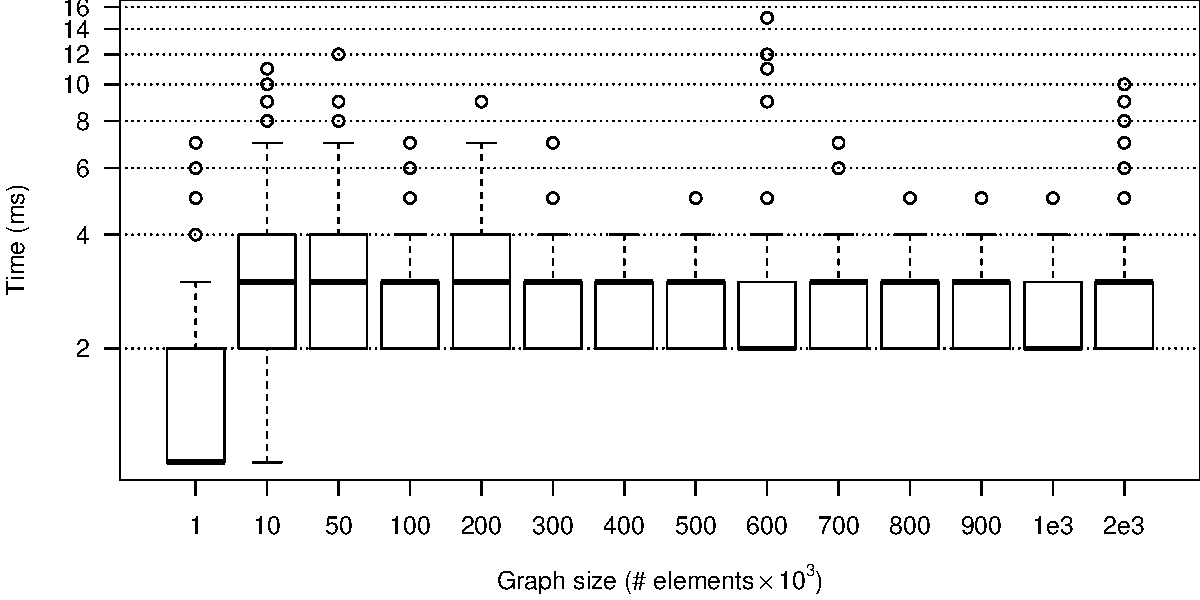
\includegraphics[width=0.85\linewidth]{img/chapt-tkm/validation/exp1-exec-log}
			\label{fig:exp1-exec}
	}
	\hfil
	\subfloat[Memory evolution] {
			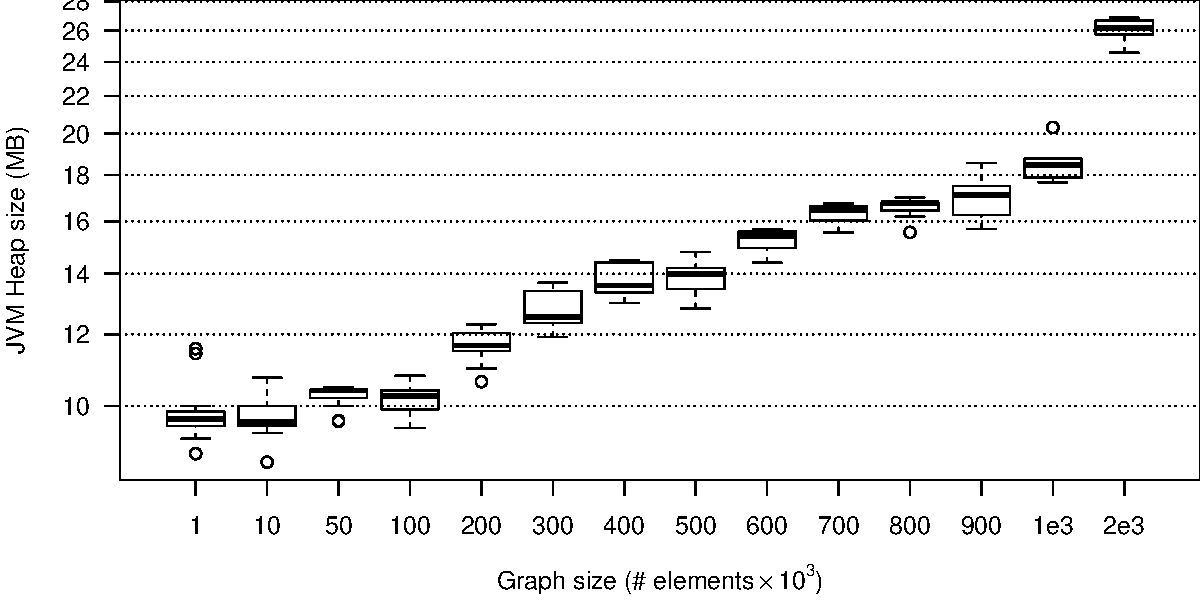
\includegraphics[width=0.85\linewidth]{img/chapt-tkm/validation/exp1-mem-log}
			\label{fig:exp1-mem}
		}	
	\caption{Experimentation results when the knowledge based size increases}
	\label{fig:exp1}
\end{figure}

\paragraph{How performance is influenced by the input size (I)?}
The second experiment aims to show the impact of the input size (I) on the execution of diagnosis algorithms. We fix the size of \textit{N} to 500\,000 and we variate \textit{I} from 1\,000 nodes to 100\,000, \ie from 0.2\% to 20\% of the graph size. 
The results are depicted in Figure~\ref{fig:exp-res} (straight lines).

Unlike to the previous experiment, we notice that the input size (\textit{I}) impacts the performance, both in terms of memory consumption and execution time. This is because our framework keeps in memory all the traversed elements, namely the input elements.
The increase in memory consumption follows a linear trend with regards to \textit{N}. As it can be noticed, it reaches 2GB for \textit{I}=100\,000. The execution time also shows a similar curve, while the query response time takes around than around 60ms to run for \textit{I}=1\,000, it takes a bit more than 4 seconds to finish for \textit{I}=100\,000. Nonetheless, these results remain very acceptable for diagnosis purposes. 

\paragraph{How performance is influenced by the number of traversed elements (M)?}%
For the last experiment, we aim to highlight the impact of the number of traversed elements (\textit{M}). For this, we fix \textit{I} and \textit{O} to 1, and randomly generate a graph with sizes ranging from $1\,000$ to $100\,000$. Our algorithm navigates the whole model (\textit{M}=\textit{N}).
We depict the results in Figure~\ref{fig:exp-res} (dashed curve).
As we can notice, the memory consumption increases in a quasi-linear way. The memory footprint to traverse \textit{M} = 100\,000 elements is around 0.9GB. The progress of the execution time curve behaves similarly, in a quasi-linear way. Finally, the execution time of a full traversal over the biggest graph takes less than 2.5 seconds. 

\begin{figure}
	\centering
	\subfloat[Evolution of the execution time]{
		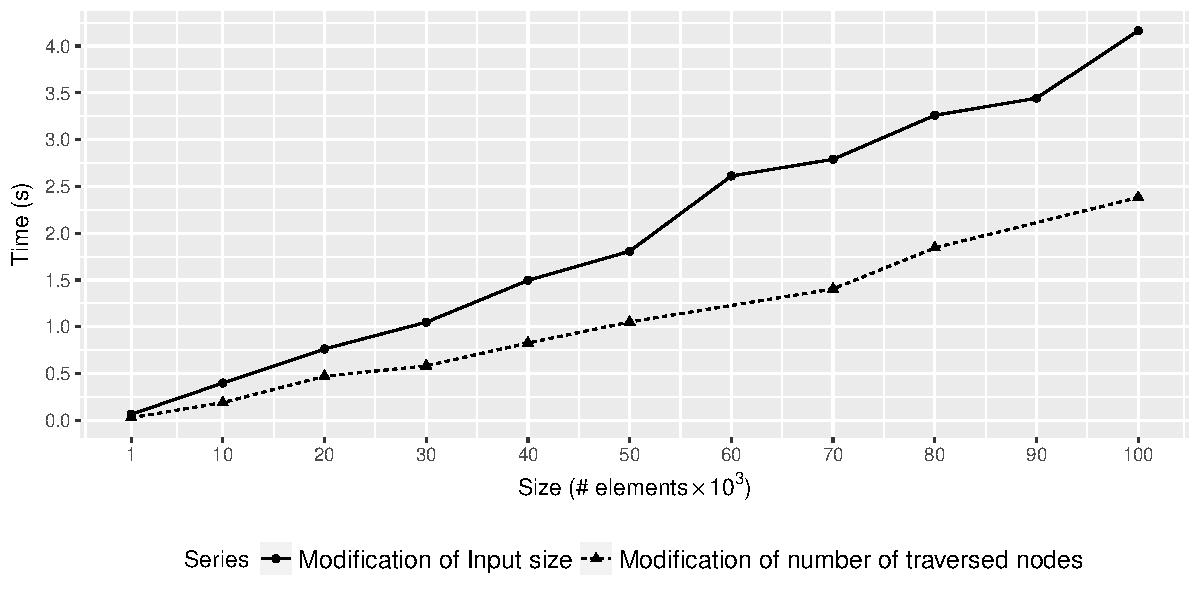
\includegraphics[width=0.9\linewidth]{img/chapt-tkm/validation/exp-exec}
		\label{fig:exp-exec}
	}
	\hfil
	\centering
	\subfloat[Evolution of the memory consumption]{
		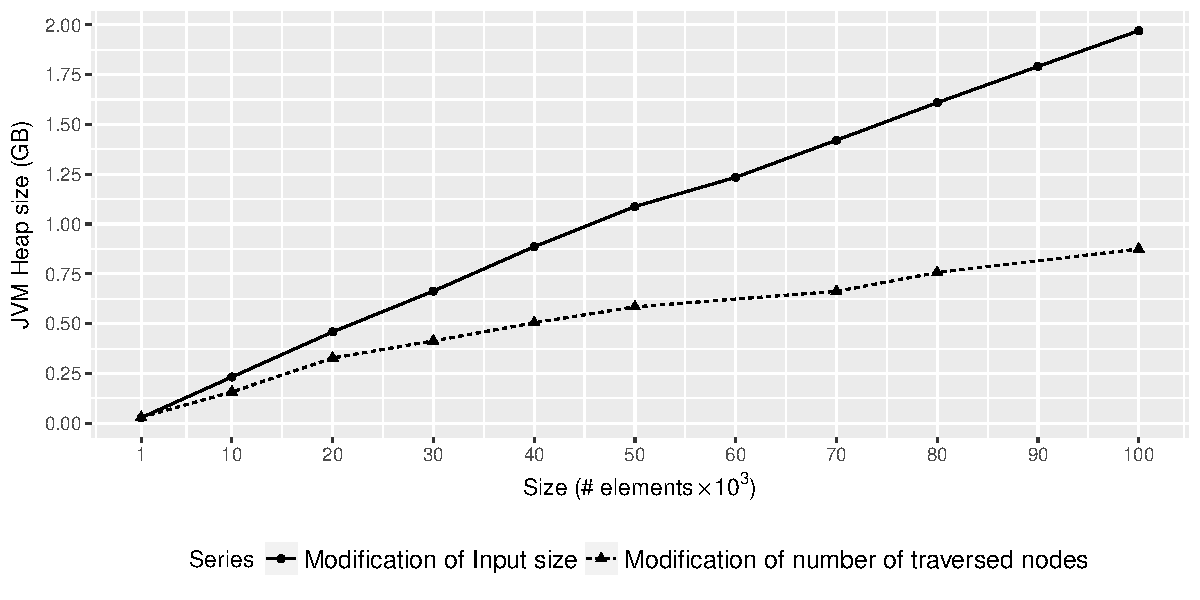
\includegraphics[width=0.9\linewidth]{img/chapt-tkm/validation/exp-mem}
		\label{fig:exp-mem}
	}
\caption{Results of experiments when the number of traversed or input elements  increases}
\label{fig:exp-res}
\end{figure}

\subsection{Discussion}
By linking context, actions, and requirements using decisions, data extraction for explanation or fault localization can be achieved by performing common temporal graph traversal operations.
In the detailed example, we show how a stakeholder could use our approach to define the different elements required by such systems, to structure runtime data, finally, to diagnose the behavior of adaptation processes. 

Our implementation allows to dynamically load and release nodes during the execution of a graph traversal. Using this feature, only the needed elements are kept in the main memory.  Hence, we can perform interactive diagnosis routines on large graphs with an acceptable memory footprint. 
However, the performance of our solution, in terms of memory and execution time, is restricted by the number of traversed elements and the number of input elements.
Indeed, as shown in our experimentation, both the execution time and the memory consumption grow linearly.

As described in~\cite{DBLP:conf/smartgridcomm/0001FKTPTR14}, the smart grid in Luxembourg is composed of 1 central system, 3 data concentrators and 227 meters.
The network is thus composed of 231 elements.
Each meter sends the consumption value every 15 min, being 908 every hours.
Plus, there is from 0 to 273 topology modifications in the network.
In total, the system generates from 908 to 1,181 new values every hour.
If we consider that we have one model element per smart grid entity and one model element per new value, 100,000 model elements correspond thus from $((100,000 - 231) * 1H ) / 1,181 = 84,5H$ ($\sim$ 3,5 days) to $((100,000 - 231) * 1H ) / 908 = 109,9H$ ($\sim$ 4,6 days) of data. In other word, our approach can efficiently interrogate up to $\sim$5 days history data in 2.4s.


 \section{Threat to validity}
\label{sec:tkm:threat2Valid}

\paragraph{Size of the model}

\paragraph{Engineer effort to use the solution}

\paragraph{Performance of the adaptation process}
 \section{Conclusion}
\label{sec:tkm:conclusion}
 
 






